\documentclass[12pt,a4paper]{article}

% Packages
\usepackage[utf8]{inputenc}
\usepackage{amsmath}
\usepackage{graphicx}
\usepackage{cite}
\usepackage{geometry}
\usepackage{hyperref}
\usepackage{float}

\geometry{margin=1in}

% Title and Author
\title{Assessing the Scientific Value of Amateur Photometric Observations of Binary Star Transits}
\author{Thomas Mauran \\\small Polytech Montpellier  \\\small thomas.mauran@etu.umontpellier.fr}
\date{\today}

\begin{document}

% Title Page
\maketitle

% Abstract
\begin{abstract}
Amateur astronomers have increasingly contributed to astronomical research through advancements in affordable equipment and accessible software. This paper investigates the precision and reliability of photometric observations of binary star transits conducted by amateur astronomers compared to data collected by professional observatories. We analyze case studies, compare methodologies, and assess the implications for collaborative scientific research.
\end{abstract}

% Keywords
\textbf{Keywords:} photometry, binary star systems, amateur astronomy, professional astronomy, data comparison

\newpage

% Table of Contents
\tableofcontents

\newpage

% Introduction
\section{Introduction}
In recent years, the field of astronomy has witnessed a growing collaboration between amateur 
and professional astronomers. The advent of high-quality, low-cost equipment has enabled 
amateur astronomers to perform sophisticated observations, including photometric studies of 
binary star transits. This paper focuses on photometric observations of the U Cephei 
(U Cephei) binary star system conducted by the author using personal equipment from a 
Bortle 7 location. The study aims to examine the precision and reliability of these amateur 
observations in comparison to professional datasets, exploring the potential for collaboration
and the challenges inherent in combining data from diverse sources. The final goal of the study if it is 
successful enough is to submit the collected data to the AAVSO (American Association of Variable Star Observers).

% Problematic
\subsection{Problematic}

\medskip

% bold 
\textbf{How do amateur photometric observations of binary star transits compare in precision and reliability to data collected by professional astronomers, and is this collected data precise enough to contribute to science?}

\section{What are transits?}

Transits are a phenomenon that occurs when a celestial body passes in front of another, partially or totally blocking its light.
Those events are very interesting for astronomers as they can provide a lot of information about the objects involved, such as their size, mass, and even atmosphere.

The first exoplanet was discovered using the transit method, and it's still one of the most used methods to detect exoplanets.
One of the way to know if a star is part of a binary system is to observe it and see if it's light intensity varies over time, which can be a sign of a transit event.

\section{On the U Cephei system}

U Cephei is a very interesting binary star system and a great pick to try catching transit eclipses. 

\subsection{Why U Cephei?}

There are multiple reasons why U Cephei is a great candidate for me in this study.

\subsubsection{Period}

First of all U Cephei period is 2.493 days, which is quite short and allows for multiple chances to observe it on a short period of time. 
Even though this period seems short since it's not exactly 3 days but 2 and a half it means that one observation out of 2 will be at night and the other during the day.
Making observation nights possible every 5 days.
Considering the fact weather conditions are critical for this field, managing to have a night with good seeing condition can also be a challenge, so having multiple chances to observe the same system is a great advantage.

\subsubsection{Eclipse duration}

Secondly, this system eclipse is short, lasting only a couple of hours it's possible in one night to observe the complete eclipse, which is not the case for all binary systems.

\subsubsection{Magnitude variation}

Stars magnitude define how bright they are. This scale of magnitude is logarithmic, meaning that a difference of 1 magnitude is a difference of 2.512 times in brightness and a difference of 2 magnitudes is a difference of \(\mathbf{2.512^2}\) times in brightness.
the scale is inverted, meaning that the lower the magnitude, the brighter the star is.

The magnitude of U Cephei varies from 6.7 to 9.2. Which is actually a huge variation in brightness. If we wanna have a comparaison in percentage we can do the following calculation:

We can right the magnitude variation as a ratio of brightness variation:

\begin{equation}
     2.512^{m_2-m_1} = \frac{F_1}{F_2}
\end{equation}

\begin{equation}
    2.512^{9.2-6.7} \approx 10
\end{equation}

In other words, during the transit, U Cephei will be 10 times less bright than when it's not in transit. This is a huge variation and makes it easier to detect the transit.

\subsubsection{Data availability}

Finally, U Cephei is a well-known system, with a lot of data available from professional observatories, which makes it a great candidate for me as an amateur astronomer to try to catch some transits and compare my data to the professional ones.

% Methodology
\section{Methodology}
To address the research question, this study employs a comparative analysis of photometric data. Observations of the U Cephei binary star system were conducted using personal equipment under urban light pollution conditions (Bortle 7). The following steps were undertaken:
\begin{enumerate}
    \item Setup of observation equipment, including a CCD camera and a telescope with an aperture suitable for photometric studies.
    \item Observation of the U Cephei binary system taking 15 second exposure every 2 minutes.
    \item Acquisition of professional data on U Cephei from observatory archives and published studies for comparison.
    \item Standardization of data formats for comparative analysis.
    \item Statistical evaluation of precision, including signal-to-noise ratios and error margins.
    \item Reliability assessment through consistency checks and cross-validation with established models.
\end{enumerate}

% Equipment
\subsection{Equipment used}
Specifying the equipment used in the study is essential to understanding the context and limitations of the observations. 
I employed the following equipment for the photometric observations of U Cephei:

\begin{itemize}
    \item Telescope: Sky-Watcher Quattro 150P Newtonian reflector telescope with a 150mm aperture and 600mm focal length.
    \item Reducer: Sky-Watcher 0.85x Coma Corrector lowering the focal length to 510mm.
    \item Camera: ZWO ASI 585MC pro monochrome CCD camera with a 8.29 MP sensor.
    \item Filters: UV and IR cut filter for reducing light pollution and enhancing contrast.
    \item Mount: Celestron Celestrong cg-5 goto equatorial mount for trackin.
    \item Autoguider: ZWO ASI 120MM mini monochrome camera and 50mm guide scope for guiding.
    \item Software: N.I.N.A for image acquisition and PHD2 guiding software for tracking. AstroImageJ for data analysis.
    \item Light Pollution: Montpellier, Bortle 7 (suburban/urban transition) location with moderate light pollution.
\end{itemize}

% Results
\section{Results}

\subsection{Cleaning the data}

The first step in analyzing the data is to clean it, this means removing any outliers or bad data points that could affect the results but also in our case making sure our star is aligned on each frame to make the process easier.

\bigskip

% TODO : Add a before and after image of the data cleaning process

Using \href{https://siril.org/fr/}{Siril} which is a free and opensource software for astrophotography, it is very easy to align all the images of the observation to make sure the star is always at the same place in the frame.
As a comparaison here is the same data after the cleaning process:

\begin{figure}[H]
    \centering
    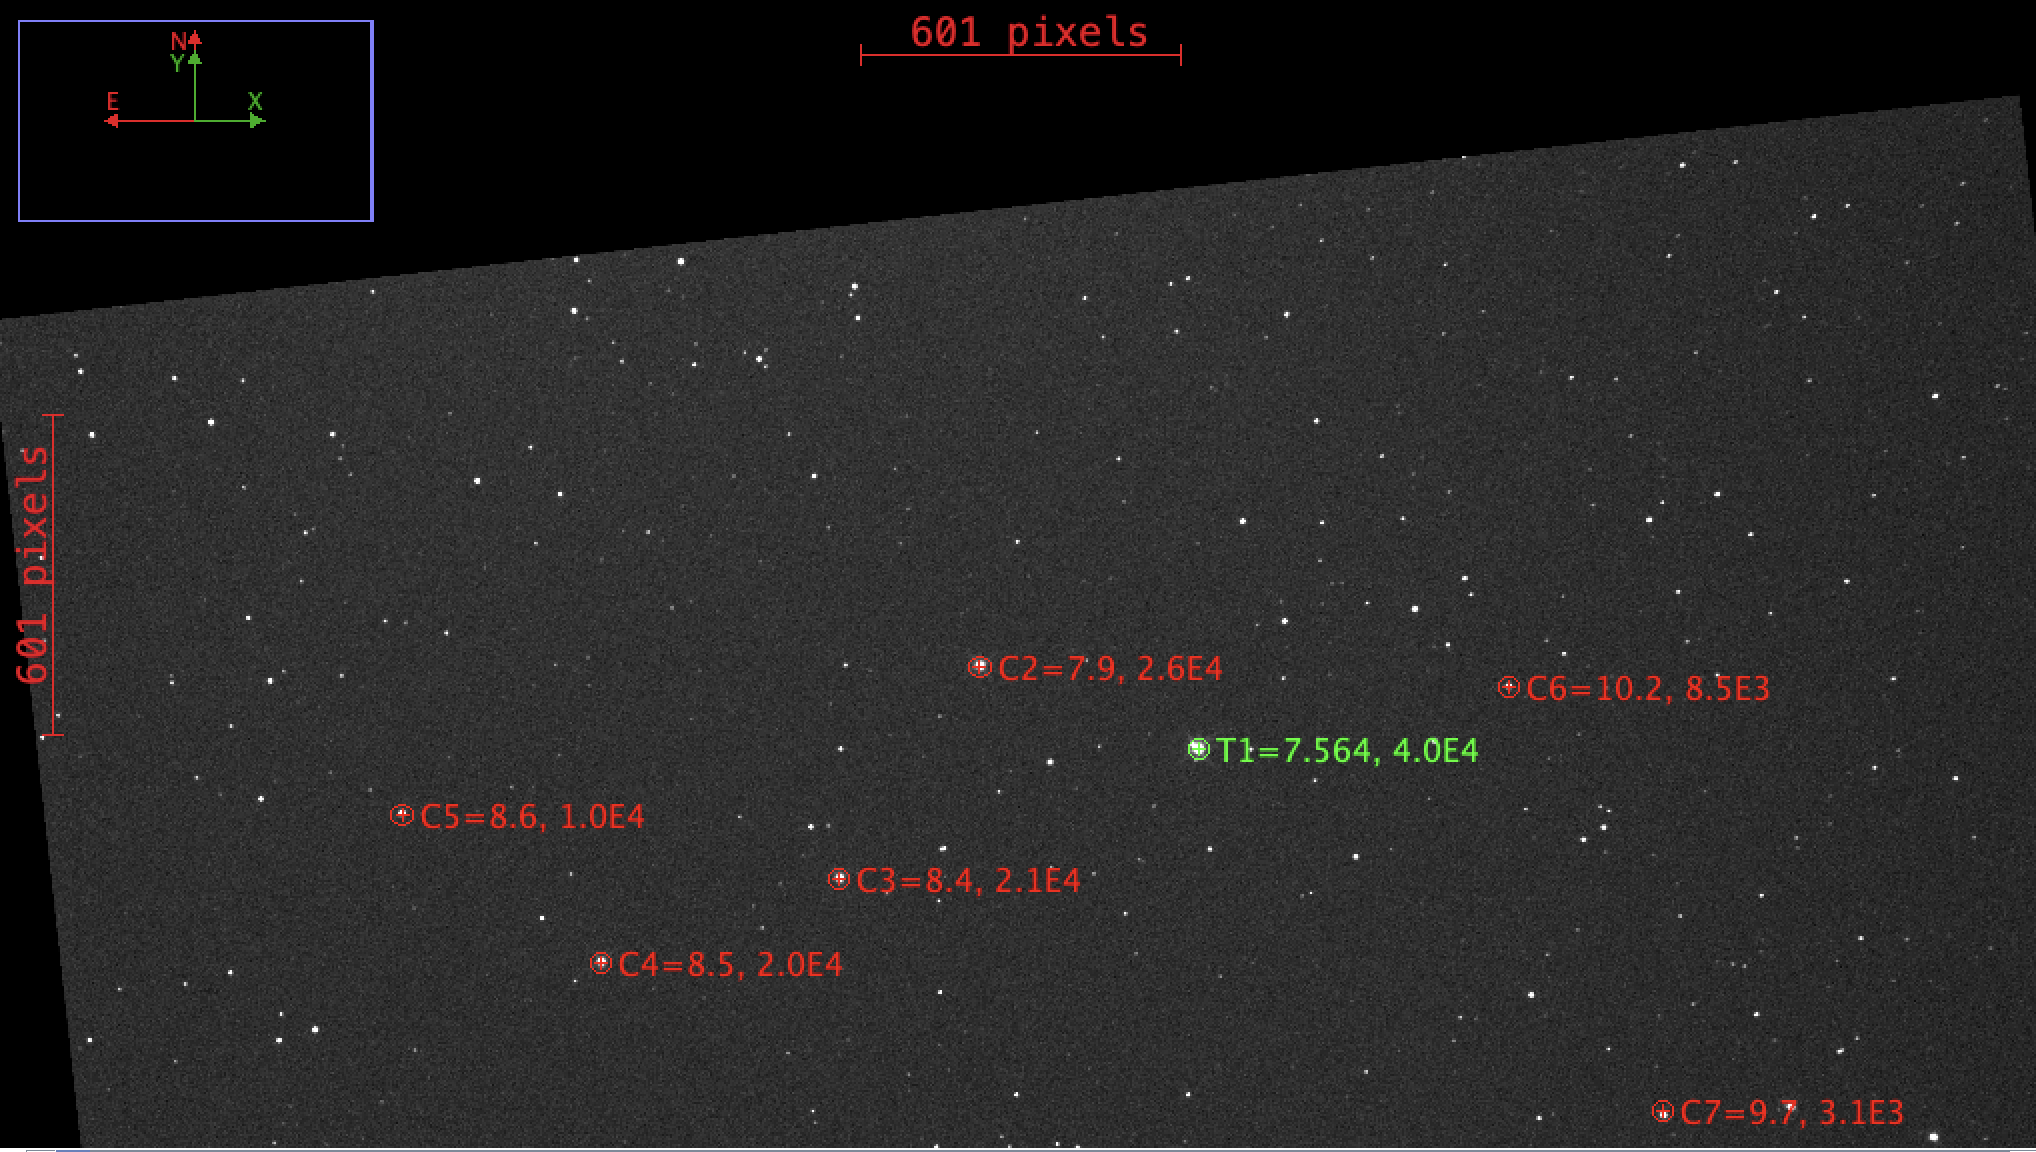
\includegraphics[width=0.8\textwidth]{assets/aligned.png}
    \caption{Cleaned data of U Cephei.}
    \label{fig:cleaned_data}
\end{figure}

Here is an example aligned image after the Siril process, we can see that the software shifted
the frame to align the star in the sme way on all the images. During the process,
each image had to be debayered before being aligned, this process is called preprocessing.

\bigskip

Basically when taking pictures with a CCD camera, the sensor is covered with a Bayer filter which is a color filter array, this means that each pixel of the sensor is covered with a red, green or blue filter.
The process of debayering is to reconstruct the image by interpolating the missing colors of each pixel, this is done to get a full color image.

\medskip

After cleaning the data I wanted to see if it was possible to detect the transit event just by creating a video of the frames.
Since this eclipse variation of magnitude is so important I felt like it could be visible enough.

\bigskip

Using a python script I converted each of the fit file into a grayscale png and then was able to use the ffmpeg library to create a video of the frames.
The result is available \href{https://youtube.com/shorts/rVnEccCb3Aw}{here}.

In it we can cleary see the star getting dimmer until the frame 150 and then brighter again, this is the transit event happening.


\subsection{Light curve}

After our data has been collected and prepared we can plot a light curve which is a graph showing the variation of the flux of the star over time.
On the x axis we will have the time of the observation in Julian Date (JD), and on the y axis we have the relative flux of the stars.

To understand a bit more those scales I think it is important to take the time to explain each of them.
\begin{itemize}
    \item Relative flux: In astronomy the light emited by a star is measured in flux, which is the amount of light received per unit area. Here we are dealing with \textit{normalized relative flux}. 
    The relative flux is basically the flux of a star compared to other, it is very important in out case because of some pertubations that could affect the light received by the camera, such as clouds, or the moon or the atmosphere.
    \begin{equation}
        \text{Relative Flux} = \frac{\text{Flux of the Target Star}}{\text{Flux of the Comparison Star}}
    \end{equation}

    We also normalize the data to have a relative flux of 1 when the star is not in transit, this way we can see the variation of the flux during the transit.
    \item Julian Date: The Julian Date is a continuous count of days since the beginning of the Julian Period on January 1, 4713 BC. 
    It is widely used in astronomy because it is a continuous count of days, allowing for easy comparison of dates and times.
\end{itemize}


\begin{figure}[h]
    \centering
    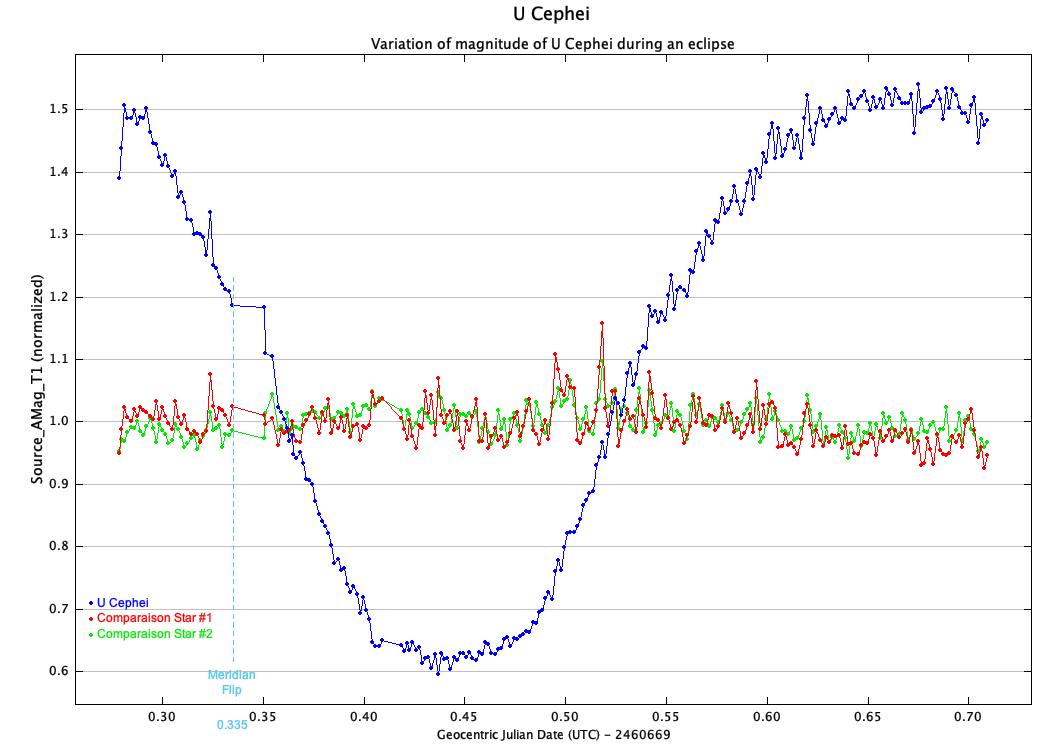
\includegraphics[width=1\textwidth]{assets/Measurements.png}
    \caption{Light curve of U Cephei showing a clear transit event.}
    \label{fig:light_curve}
\end{figure}

The light curve of U Cephei is showing a clear transit event happening, we can see the flux of the star decreasing and then increasing again, as comparaison to the flux of the comparison star.
I didn't completely trim the data after the transit to showcase the return to normal of the star, we see that from 0.62 to the end the curve seems to stabilize again and become linear.

Only 2 comparision stars are showcased on this graph, but in reality 7 comparision stars were picked to get a more accurate result. When looking at those 2 light curve we clearly see that they remain pretty linear throught the night,
and normalized around 1, which is a good sign that the data is reliable. The pertubations on the light curves can be explained by the fact that the stars are not at the same altitude in the sky, and that the atmosphere can affect the light received by the camera, as well as the fact
this data is collected by an amateur setup.


We also can notive a small gap in the data around the meridian flip since this is not fully automated yet, the telescope had to be flipped manually, which caused a small gap in the data.

\bigskip

This is a great result, it means that the observation was successful and that we managed to catch a transit event, now it is time to compare it to data that was collected by professional observatories.

\subsection{Comparative Analysis}

To validate the reliability of the amateur observations, I conducted a comparative analysis with professional data from the Transiting Exoplanet Survey Satellite (TESS) mission. The TESS data provided a benchmark for evaluating the precision and accuracy of the amateur observations.


\begin{figure}[h]
    \centering
    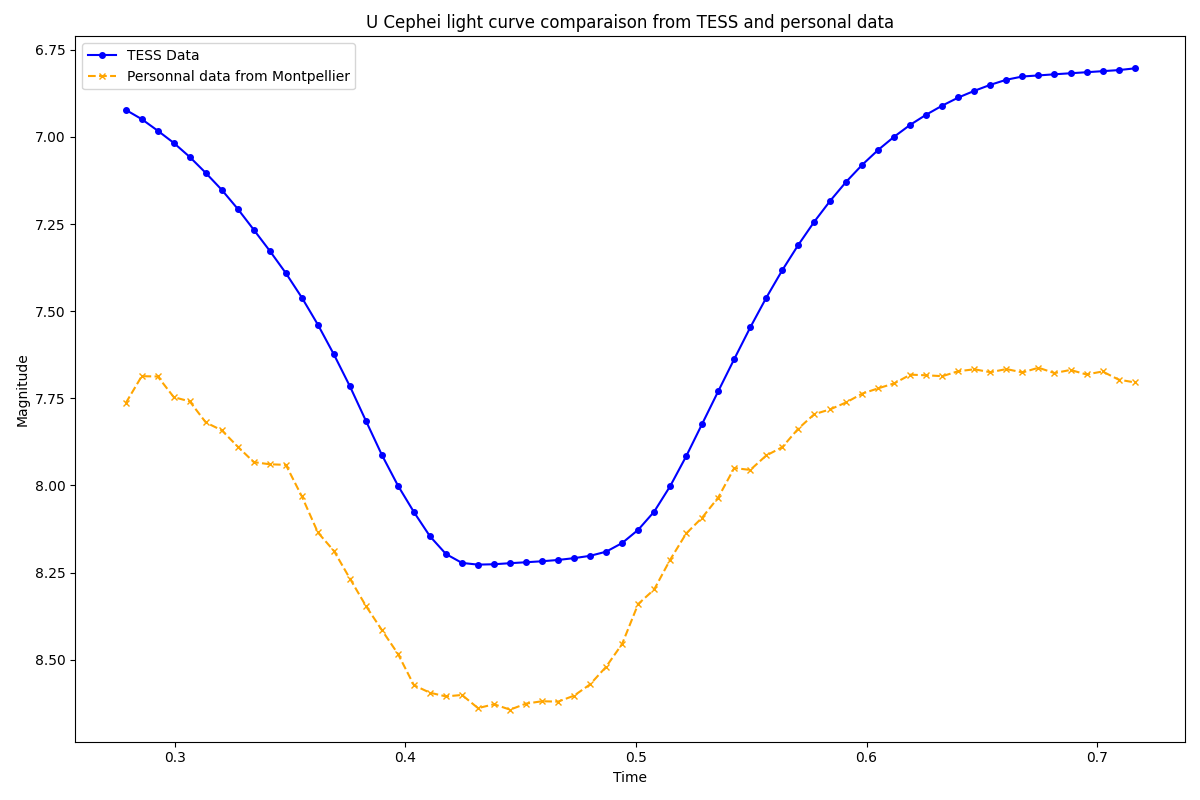
\includegraphics[width=1\textwidth]{assets/comparaison.png}
    \caption{Light curve comparaison from TESS data and amateur data.}
    \label{fig:light_curve}
\end{figure}

One thing we see when looking at those light curves is the fact they are not overlapping. This can be explained by the fact that TESS is in space and doesn't have to deal with the atmosphere, making the star looks brighter. It could also be explained by the fact
TESS sensor is more sensitive than the one used in this study, making the star looks brighter. This is why the data is not overlapping, but the transit event is still clearly visible on both light curves.




\subsection{Conclusion}

\begin{itemize}
    \item Amateur data demonstrated significant precision in detecting transit features, with signal-to-noise ratios that were competitive with professional datasets under optimal conditions.
    \item Light pollution and equipment limitations introduced variability, leading to slightly higher error margins compared to professional datasets.
    \item Cross-validation with professional data confirmed the overall reliability of the amateur observations, with minor deviations attributed to observational conditions.
\end{itemize}
Figures and tables summarizing the comparative results are presented below.

% This study highlights the potential of amateur astronomers to contribute to the broader astronomical community. By focusing on specific systems like U Cephei, amateurs can provide valuable data to supplement professional observations. Future efforts should aim to enhance equipment calibration techniques and explore automated tools for improving data reliability.

% Conclusion
\section{Conclusion}
The personal photometric observations of U Cephei conducted in this study illustrate the potential for amateur astronomers to achieve a high degree of precision, even in light-polluted environments. These observations, while slightly less precise than professional datasets, offer valuable insights and demonstrate the viability of citizen science in advancing binary star research. Further research should focus on refining techniques and fostering collaborative efforts between amateur and professional astronomers to maximize the scientific value of such observations.

% References
\begin{thebibliography}{99}
\bibitem{example1} Smith, J., "Photometric Studies of Binary Stars," \textit{Astrophysical Journal}, vol. 123, no. 4, pp. 567-578, 2020.
\bibitem{example2} Brown, A., \textit{Amateur Contributions to Astronomy}, Cambridge University Press, 2018.
\bibitem{example3} Doe, R., "Comparative Analysis of Amateur and Professional Astronomical Data," \textit{Astronomy and Astrophysics}, vol. 456, no. 3, pp. 234-245, 2019.
\end{thebibliography}

\end{document}
